\documentclass{article}
\usepackage[utf8]{inputenc}
\usepackage{amsmath}
\usepackage{amssymb}
\usepackage{graphicx}
\graphicspath{{Images/}}

\setlength{\oddsidemargin}{0in}
\setlength{\textwidth}{6.5in}
\setlength{\topmargin}{-.55in}
\setlength{\textheight}{9in}
\pagestyle{empty}

\title{Scientific Computation HW2}
\author{Michael Nameika}
\date{September 2022}

\begin{document}
 
\maketitle


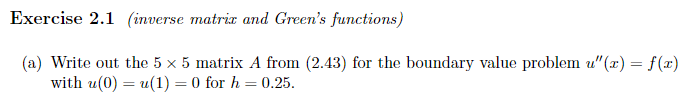
\includegraphics[scale = 0.75]{prob1a.PNG}
\newline\newline

Using the form of the matrix in (2.43) for $h = 0.25$, we get
\[A = \frac{1}{0.25^2}
\begin{bmatrix}
    0.25^2 & 0 & 0 & 0 & 0\\
    1 & -2 & 1 & 0 & 0\\
    0 & 1 & -2 & 1 & 0\\
    0 & 0 & 1 & -2 & 1\\
    0 & 0 & 0 & 0 & 0.25^2\\
\end{bmatrix}\]
\[=
\begin{bmatrix}
    1 & 0 & 0 & 0 & 0\\
    16 & -32 & 16 & 0 & 0\\
    0 & 16 & -32 & 16 & 0\\
    0 & 0 & 16 & -32 & 16\\
    0 & 0 & 0 & 0 & 1\\
\end{bmatrix}\]


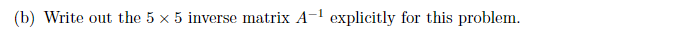
\includegraphics[scale = 0.75]{prob1b.PNG}
\newline\newline
Solving for the inverse of $A$, we find
\[A^{-1} = \begin{bmatrix}
    1 & 0 & 0 & 0 & 0\\
    3/4 & -3/64 & -1/32 & -1/64 & 1/4\\
    1/2 & -1/32 & -1/16 & -1/32 & 1/2\\
    1/4 & -1/64 & -1/32 & -3/64 & 3/4\\
    0 & 0 & 0 & 0 & 1\\
\end{bmatrix}\]

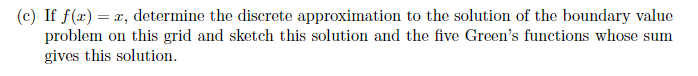
\includegraphics[scale = 0.75]{prob1c.PNG}
\newline\newline

We will approximate $x$ on the interval $[0,1]$ by the following sum of Dirac Delta functions: $x \approx 0\delta(x) + \frac{1}{4}\delta(x - 1/4) + \frac{1}{2}\delta(x - 1/2) + \frac{3}{4}\delta(x - 3/4) + \delta(x - 1)$. That is, we are approximating $x$ on $[0,1]$ with a mesh grid of mesh width $1/4$. Using this approximation, our differential equation turns into
\[U''(x) = \frac{1}{4}\delta(x - 1/4) + \frac{1}{2}\delta(x - 1/2) + \frac{3}{4}\delta(x - 3/4) + \delta(x - 1)\]
Where $U(x)$ denotes the approximate solution and $u(x)$ denotes the exact solution.

And we know that for any linear operator $\mathcal{L}$, $\mathcal{L}(G(x,\bar{x})) = \delta(x - \bar{x})$ and by the superposition principle, we have 
\[\mathcal{L}(G(x, \bar{x}_1) + G(x, \bar{x}_2) + \cdot \cdot\cdot + G(x, \bar{x}_n)) = h\delta(x - \bar{x}_1) + h\delta(x - \bar{x}_2) + \cdot\cdot\cdot + h\delta(x - \bar{x}_n)\]
So we expect that our solution to our discretized differential equation will be of the form
\[U(x) = h\frac{1}{4}G(x, 1/4) + h\frac{1}{2}G(x,1/2) + h\frac{3}{4}G(x,3/4) + hG(x, 1)\] 
where 
\[G(x, \bar{x}) = \begin{cases}
    x(\bar{x} - 1) & 0 \leq x \leq \bar{x}\\
    \bar{x}(x - 1) & \bar{x} \leq x \leq 1\\
\end{cases}\]
The following figure shows the scaled Green's functions as they appear in the above equation:

\begin{center}
    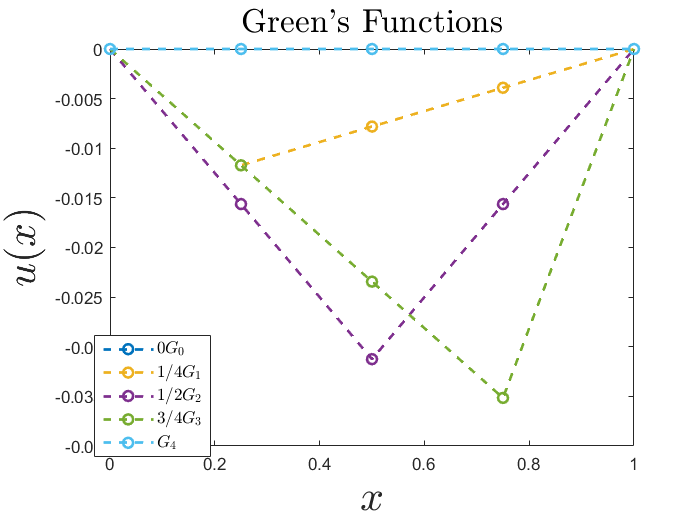
\includegraphics[scale = 0.5]{greensfunctionsfixed.png}
\end{center}

And their sum $U(x)$ plotted against the exact solution $u(x) = \frac{1}{6}x^3 - \frac{1}{6}x$:
\begin{center}
    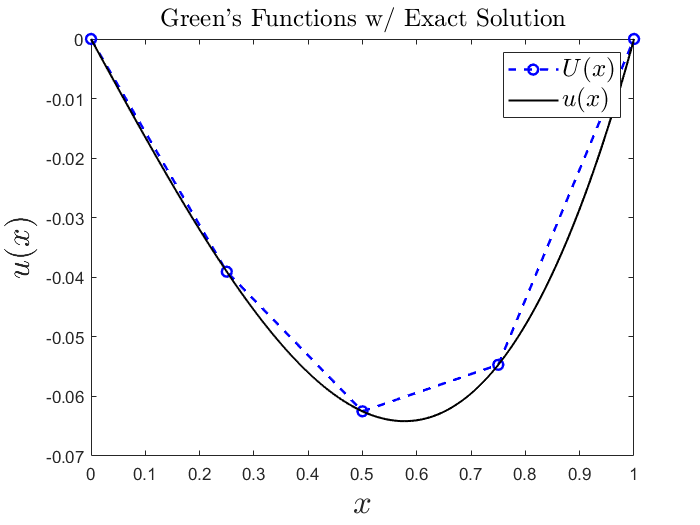
\includegraphics[scale = 0.5]{approximate with exact.png}
\end{center}

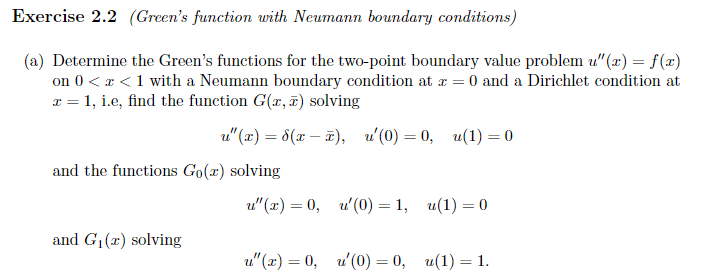
\includegraphics[scale = 0.75]{prob2a.PNG}
\newline\newline

We wish to find Green's function that satisfies $G''(x,\bar{x}) = \delta(x - \bar{x})$ with boundary conditions $G'(0,\bar{x}) = 0$, $G(1,\bar{x}) = 0$. Integrating the above differential equation, we get
\[G'(x,\bar{x}) = \begin{cases}
    c_1, & 0 \leq x \leq \bar{x}\\
    c_2 + 1, & \bar{x} \leq x \leq 1\\
\end{cases}\]
Evaluating the above expression at $x = 0$, we find $c_1 = 0$ from the given boundary conditions. Now, integrating again, we get the following:
\[G(x,\bar{x}) = \begin{cases}
    c_3 & 0 \leq x \leq \bar{x}\\
    (c_2 + 1)x + c_4 & \bar{x} \leq x \leq 1\\
\end{cases}\]
Evaluating the above expression at $x = 1$, we get $c_2 + 1 + c_4 = 0$ from the given boundary condition. Solving for $c_4$, we get $c_4 = -(c_2 + 1)$. Substituting this back in, we find
\[G(x, \bar{x}) = \begin{cases}
    c_3 & 0 \leq x \leq \bar{x}\\
    (c_2 + 1)(x - 1) & \bar{x} \leq x \leq 1\\
\end{cases}\]
Additionally, we require that $G'(x, \bar{x})$ must have a jump of 1 at $\bar{x}$. That is, 
\[c_2 + 1 - 0 = 1\]
so $c_2 = 0$. Finally, we require $\lim_{x \to \bar{x}^-} G(x, \bar{x}) = \lim_{x \to \bar{x}^+} G(x, \bar{x})$. Doing this, we find 
\[c_3 = \bar{x} - 1\]
Putting it all together, we have
\[G(x, \bar{x}) = \begin{cases}
    \bar{x} - 1 & 0 \leq x \leq \bar{x}\\
    x - 1 & \bar{x} \leq x \leq 1\\
\end{cases}\]
 Now must find the solutions $G_0$ and $G_1$. From the differential equation, it is easy to see that
 \[G_0(x) = c_1x + c_2\]
 and from our boundary conditions, we have
 \[G_0(x) = x - 1\]
 similarly for $G_1(x)$:
 \[G_1(x) = 1\]
 
 
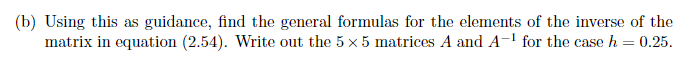
\includegraphics[scale = 0.75]{prob2b.PNG}
\newline\newline

From (2.54) for $h = 0.25$, we find
\[A = \begin{bmatrix}
    -4 & 4 & & & \\
    16 & -32 & 16 & & \\
     & 16 & -32 & 16 & \\
     & & 16 & -32 & 16\\
     & & & 0 & 1\\
\end{bmatrix}\]
We may easily compute $A^{-1}$ in MATLAB, but we may also compute $A^{-1}$ by using what we found for $G(x,\bar{x})$. To do so, notice from (2.54) that 
\[\begin{bmatrix}
    U_0\\
    U_1\\
    U_2\\
    U_3\\
    U_4\\
\end{bmatrix} = A^{-1}
\begin{bmatrix}
    \sigma \\
    f(x_1)\\
    f(x_2)\\
    f(x_3)\\
    \beta\\
\end{bmatrix}\]
Additionally, if we approximate our differential equation with Dirac Delta functions, we may say
\[U''(x) = h(f(x_1)\delta(x - x_1) + f(x_2)\delta(x - x_2) + f(x_3)\delta(x - x_3) + f(x_4)\delta(x - x_4))\]
I exclude the point $x_0$ since the value of $U'(x_0)$ is prescribed, not $U(x_0)$. Then we find the general solution to be given by
\[U(x) = h(f(x_1)G(x,x_1) + f(x_2)G(x,x_2) + f(x_3)G(x, x_3) + f(x_4)G(x,x_4)) + \sigma G_0(x) + \beta G_1(x)\]
Now, let's evaluate $U(x)$ at each $x_j$ and $U'(x)$ at $x_0$:
\[U'(x_0) = \sigma\]

\[U(x_1) = h(f(x_1)G(x_1,x_1) + f(x_2)G(x_1, x_2) + f(x_3)G(x_1,x_3) + f(x_4)G(x_1,x_4)) + \sigma (x_1 - 1) + \beta\]
\[ = - \frac{3}{16}f(x_1) - \frac{1}{2}f(x_2) - \frac{1}{8}f(x_3) - \frac{1}{16}f(x_4) - \sigma + \beta\]

\[U(x_2) = h(f(x_1)G(x_2, x_1) + f(x_2)G(x_2, x_2) + f(x_3)G(x_2, x_3) + f(x_4)G(x_2, x_4)) + \sigma (x_2 - 1) + \beta\]
\[= -\frac{3}{16}f(x_1) - \frac{1}{8}f(x_2) - \frac{1}{16}f(x_3) - \frac{3}{4}\sigma  + \beta\]

\[U(x_3) = h(f(x_1)G(x_3,x_1) + f(x_2)G(x_3,x_2) + f(x_3)G(x_3,x_3) + f(x_4)G(x_3,x_4)) + \sigma (x_3 - 1) + \beta\]
\[ = -\frac{1}{8}f(x_1) - \frac{1}{8}f(x_2) - \frac{1}{16}f(x_3) - \frac{1}{2}\sigma + \beta\]

\[U(x_4) = h(f(x_1)G(x_4,x_1) + f(x_2)G(x_4,x_2) + f(x_3)G(x_4,x_3) + f(x_4)G(x_4,x_4)) + \sigma (x_4 - 1) + \beta\]
\[ = \beta\]

Knowing that this linear system must be equal to $A^{-1}\textbf{f}$, we find the following expression for $A^{-1}$:
\[A^{-1} = \begin{bmatrix}
    -1 & -3/16 & -1/8 & -1/16 & 1\\
    -3/4 & -3/16 & -1/8 & -1/16 & 1\\
    -1/2 & -1/8 & -1/8 & -1/16 & 1\\
    -1/4 & -1/16 & -1/16 & -1/16 & 1\\
    0 & 0 & 0 & 0 & 1\\
\end{bmatrix}\]




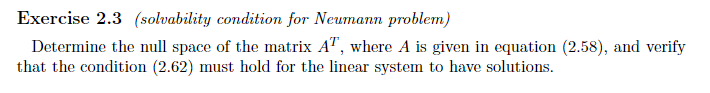
\includegraphics[scale = 0.75]{prob3.PNG}
\newline\newline

We wish to find the null space (kernel) for 
\[A^T = \begin{bmatrix}
    -h & 1 & & & & & \\
    h & -2 & 1 & & & & \\
     & 1 & -2 & 1 & & & \\
     & & 1 & -2 & 1 & & \\
     & & & \ddots & \ddots & \ddots & \\
     & & & & 1 & -2 & h\\
     & & & & & 1 & -h\\
\end{bmatrix}\]
Essentially, we are looking for all vectors $\textbf{v}$ such that $A^T \textbf{v} = \textbf{0}$. Well, solving row-by-row, we find the following equations:
\[hv_1 = v_2\]
\[v_2 = v_3\]
\[v_3 = v_4\]
\[\vdots\]
\[v_{n-2} = v_{n-1}\]
\[v_{n-1} = hv_n\]
That is, for $\textbf{v} \in \ker (A^T)$,
\[\textbf{v} = t \begin{bmatrix}
    1\\
    h\\
    \vdots\\
    h\\
    1
\end{bmatrix}\]
where $t \in \mathbb{R}$. Explicitly, we can write the kernel of $A^T$ as
\[\ker(A^T) = \left\{ t\begin{bmatrix}
    1\\
    h\\
    \vdots\\
    h\\
    1\\
\end{bmatrix} \:\: \middle| \:\: t \in \mathbb{R} \right\}\]
Now, recall the Fredholm Alternative Theorem. In order for the system $A\textbf{x} = \textbf{b}$ to have a solution, it must be true that $\textbf{b} \in \ker(A^T)^{\perp}$. That is, $\textbf{b}$ must be orthogonal to the null space of $A^T$. For our problem,
\[\textbf{b} = \begin{bmatrix}
    \sigma_0 + \frac{h}{2}f(x_0)\\
    f(x_1)\\
    f(x_2)\\
    \vdots\\
    f(x_m)\\
    -\sigma_1 + \frac{h}{2}f(x_{m+1})\\
\end{bmatrix}\]
Since $\textbf{b}$ and any vector in $\ker(A^T)$ must be orthogonal, it follows that
\[\textbf{b} \cdot \textbf{k} = 0\]
where $\textbf{k} \in \ker(A^T)$. Well, notice that the dot product with any $\textbf{k}$ will give us the following equation:
\[\sigma_0 + \frac{h}{2}f(x_0) + hf(x_1) + hf(x_2) + \cdots + hf(x_m) - \sigma_1 + \frac{h}{2}f(x_{m+1}) = 0\]
Moving $\sigma_0$ and $\sigma_1$ to the right hand side and writing the middle sum in summation notation, we get
\[\frac{h}{2}f(x_0) + h\sum_{i = 1}^mf(x_i) + \frac{h}{2}f(x_{m+1}) = \sigma_1 - \sigma_0\]
which matches equation (2.62) exactly.
\newline


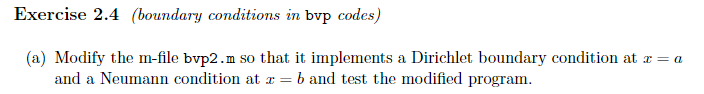
\includegraphics[scale = 0.75]{prob4a.PNG}
\newline\newline

By swapping the first and last rows of the finite difference matrix $A$, we get the effect of implementing a Neumann condition at $x = b$ and a Dirichlet condition at $x = a$ (see attached codes). For this problem, I kept the same differential equation $u''(x) = e^x$ and kept the same boundary conditions (that is, same values at the boundaries, but the type of boundary condition has changed, obviously). So our new boundary value problem is
\[u''(x) = e^x, \:\:\:\: u(0) = -5 \:\:\:\:\: u'(3) = 3\]
Which has an exact solution of
\[u(x) = e^x + (3 - e^3)x - 6\]

Running the code generates the following plots for the approximations of $u(x)$:
\begin{center}
    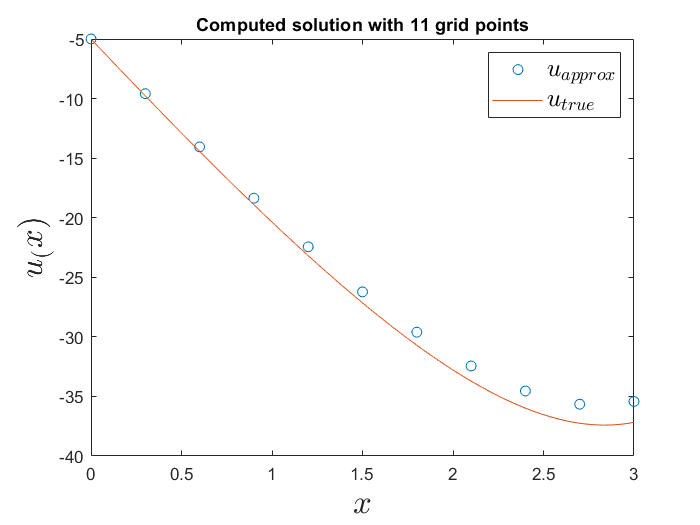
\includegraphics[scale = 0.4]{bvp2Mod_11.png}
    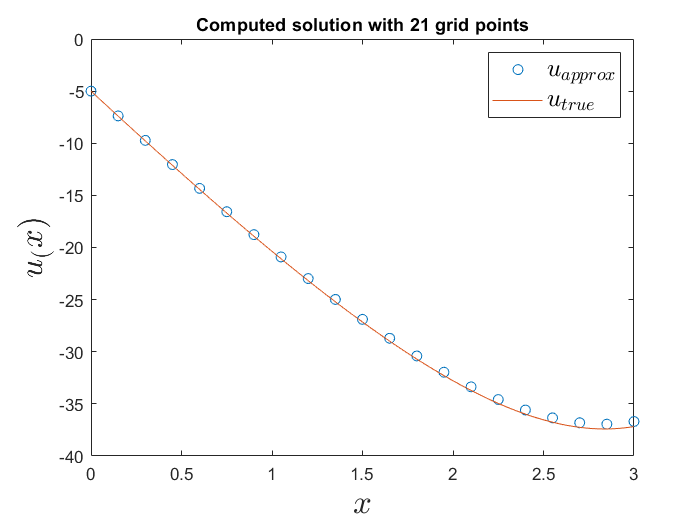
\includegraphics[scale = 0.4]{bvp2Mod_21.png}
    \newline\newline
    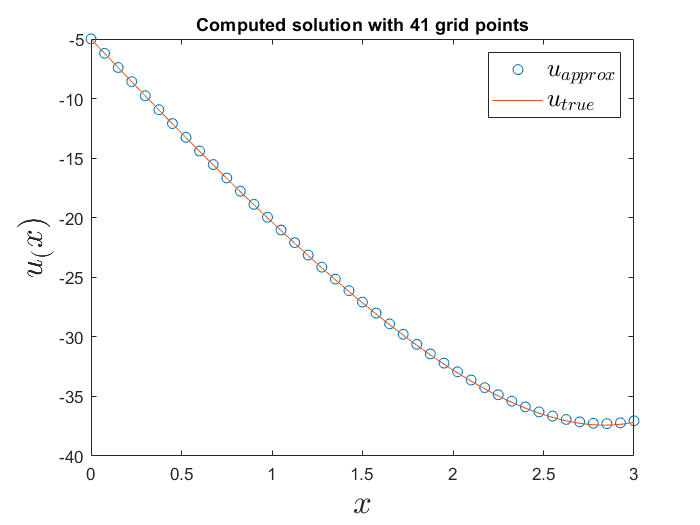
\includegraphics[scale = 0.4]{bvp2Mod_41.png}
    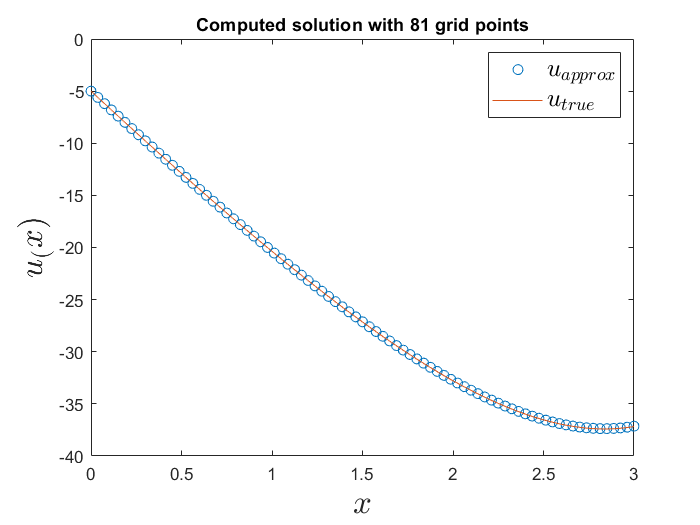
\includegraphics[scale = 0.4]{bvp2Mod_81.png}
    \newline\newline
\end{center}
With the following plot and table of the errors:
\begin{center}
    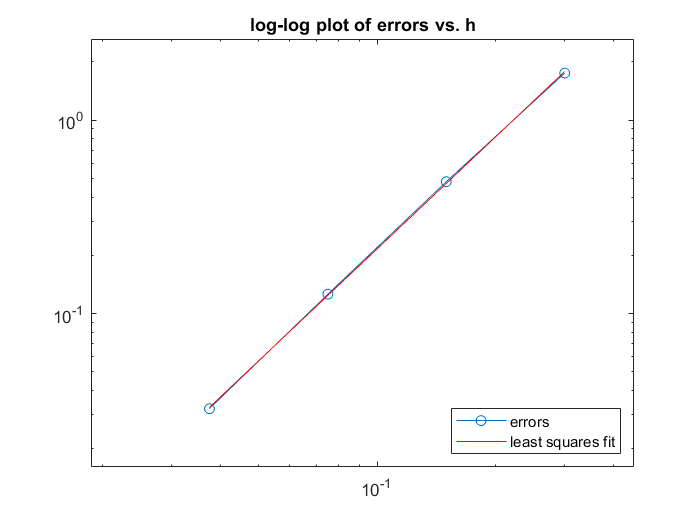
\includegraphics[scale = 0.4]{bvp2Mod_err.png}
    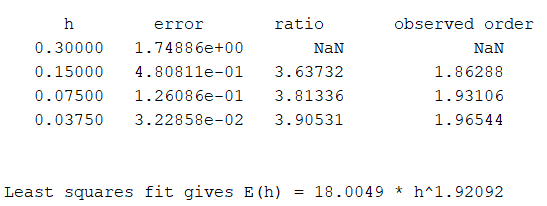
\includegraphics[scale = 0.7]{bvp2Mod_errTab.PNG}
    \newline\newline
\end{center}
Which shows that the method is approximately $\mathcal{O}(h^2)$ for this problem, as we should expect from a second order method.





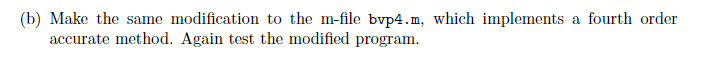
\includegraphics[scale = 0.75]{prob4b.PNG}
\newline\newline
Using the exact same process as in part (a), and utilizing the same boundary value problem, we find the following plots:
\begin{center}
    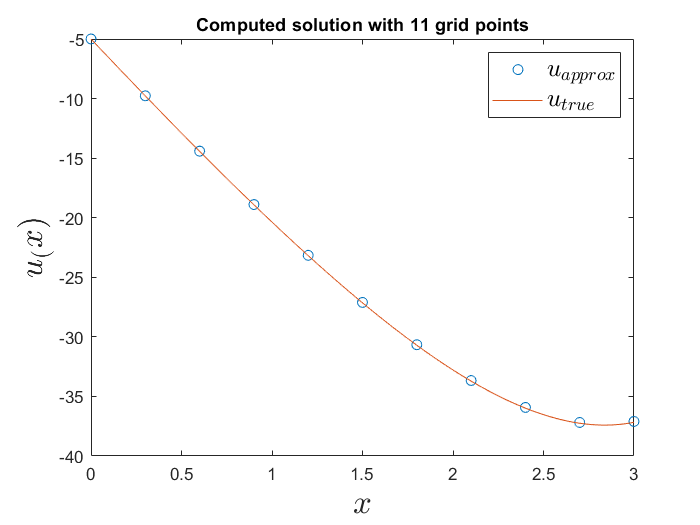
\includegraphics[scale = 0.4]{bvp4Mod_11.png}
    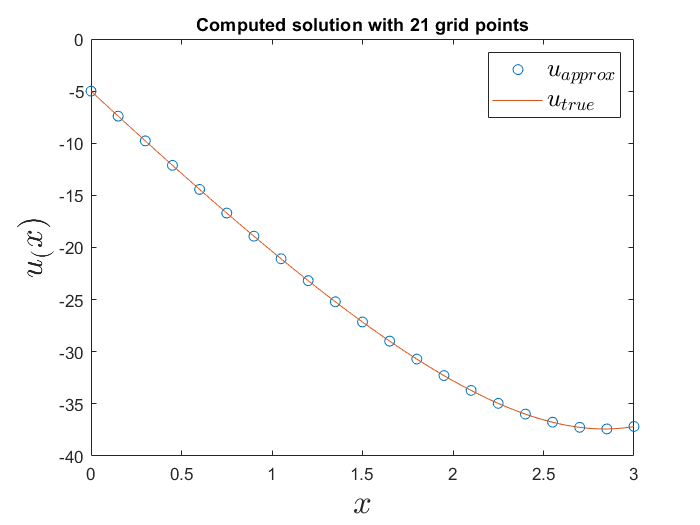
\includegraphics[scale = 0.4]{bvp4Mod_21.png}
    \newline\newline
    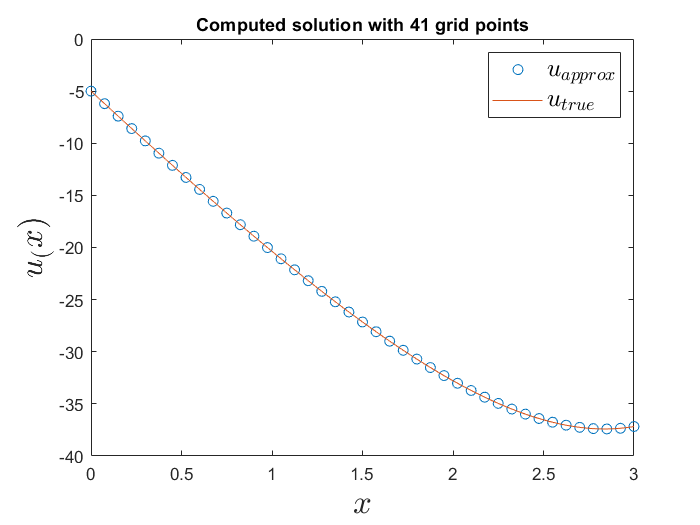
\includegraphics[scale = 0.4]{bvp4Mod_41.png}
    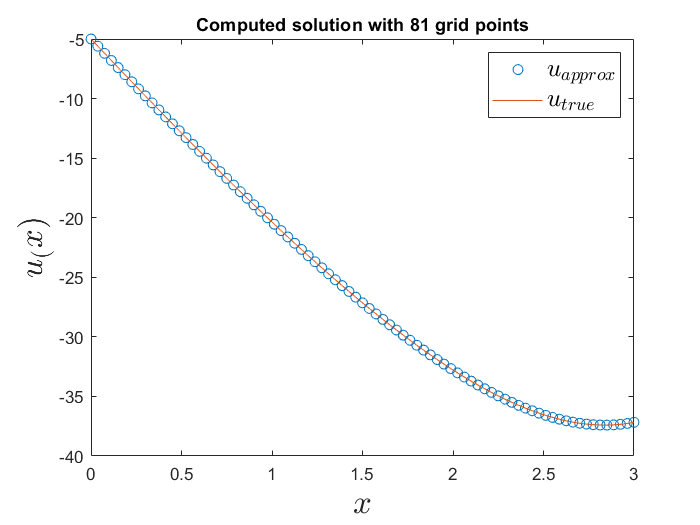
\includegraphics[scale = 0.4]{bvp4Mod_81.png}
    \newline\newline
    
\end{center}
With the following plot and table for the errors:
\begin{center}
    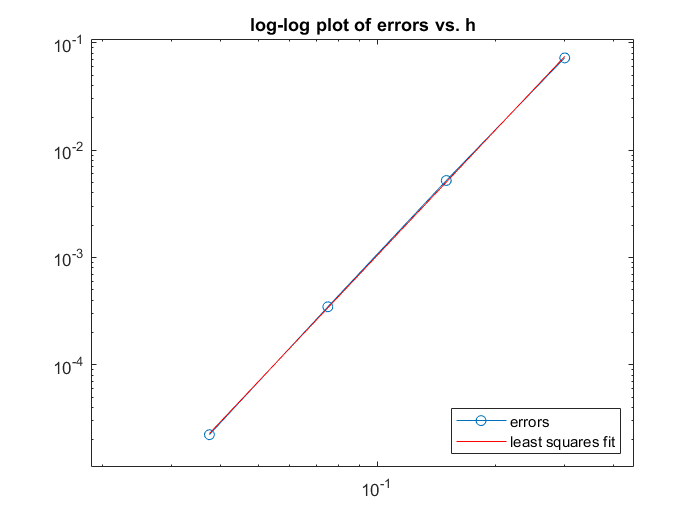
\includegraphics[scale = 0.4]{bvp4Mod_err.png}
    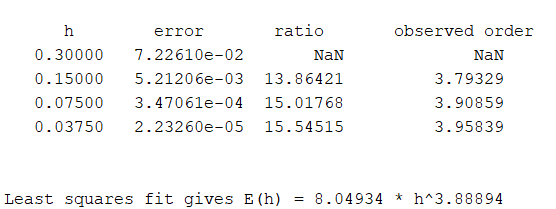
\includegraphics[scale = 0.7]{bvp4Mod_errTab.PNG}
\end{center}

We can see that this is roughly of $\mathcal{O}(h^4)$ accuracy, which is also to be expected from a fourth order method.

\end{document}
